
\section{Spatial Explanations}

To decide whether an {\explanation} is useful or not, we define two main metrics, namely intensity and influence. 

{\bf Intensity:} We define intensity as a metric that measures the {\fact} value of the explanation (the subset of dataset). Given a {\fact} $Q$ to be explained, the intensity of an {\explanation} $\phi$ can be as follows:
$$intensity = dir \cdot (Q (D_\phi) - Q(D)) $$
%Formal definition of relevance
where $D$ is the dataset and $D_\phi$ is the subset of the data represented by the {\explanation} $\phi$. $dir$ is 1 if the direction is high and -1 otherwise. 
The intuitive behind Intensity is as follows: a {\fact} $F$ indicates a value of $Q$ which is higher or lower than normal (direction). A good {\explanation} should have the highest deviation from the whole dataset then it can push the value of $Q$ towards the same direction. 
%The relevance metric borrows a lot from our definition of aggravation. 
%It might be convenient to think of a web search engine when we are looking at the intensity metric. When we use a search engine, we provide a search term as the query input. The search engine looks at all the pages in its database and returns the results in order of relevance. The top results in the search engine may not have a significant effect on the entire web if they were to be removed. However, the top result in the search engine has the highest relation to the data. For example, the top result for a search engine which uses tf-idf might be a page containing the highest frequency of the search term\cite{robertson2004understanding}.


\textbf{Influence:}
% What is influence
%We define influence as a metric which measures the value of the explanation compared to the entire dataset. The influence metric borrows from our definition of intervention. The influence metric measures how much the observation would be affected if we remove the data related to our explanation(the \textit{influence} of our explanation on the observation). We can use the analogy of the search engine again here. One of the earliest algorithms used by Google to rank web pages used links to other pages\cite{brin1998anatomy}. The page which was linked the most on a variety of websites was ranked higher. If you remove a highly relevant page, many other pages might not exist. Influence uses the same principle.
Influence measures how much the {\fact} would change if we remove the data represented by the {\explanation}. 
%Formal definition of influence
%Let $D$ be our dataset. Let $\phi$ be our candidate explanation. Let $R$ be the function which maps our dataset to the value of our observation. Then we can define relevance as,
It is defined as follows:
$$influence = dir \cdot (Q (D) - Q(D_{\neg \phi})) $$
where $D_{\neg \phi}$ represents remaining part of the dataset after removal of tuples in the {\explanation}. The intuitive behind influence is after removing the {\explanation} tuples, the remaining dataset should have the value of $Q$ towards the opposite direction as possible. Then it means the removal data has a high impact on $Q$. 
%The greater the value of influence, the more its impact on the observation.

\begin{table}
	\centering
	\caption{Intensity and influence for example {\explanation}s}
	\begin{tabular}{|c|c|c|c|c|}
		\hline
		PayType & \# on 22, Jan & \# on 23, Jan & Intensity & Influence\\ \hline
		% -1 * ((4000 / 25000) - 1/7) --> intensity
		% -1 * (1/7 - 1000 / 10000) --> influence
		% -1 * (1/7 - 4100 / 27000)
		% -1 * (1/7 - 4900 / 33000)
		%        1 & 25000 & 4000 & -0.02& -0.04\\ \hline
		%        2 & 8000 & 900  & 0.03& 0.009\\ \hline
		%        3 & 2000 & 100  & 0.09& 0.006\\ \hline
		1 & 282817 & 78133 & 0.010& 0.021\\ \hline
		2 & 134365 & 27789  & -0.02& -0.01\\ \hline
		3 & 1445 & 507  & -0.16& -0.0005\\ \hline
		4 & 535 & 169  & -0.13& -0.0006\\ \hline
		$\phi_S$ & 278852 &  41526 & 0.037 & 0.073\\ \hline
		Total    & 420162 & 78133 &- & - \\ \hline            
		%        Total    & 35000 & 5000  &- & - \\ \hline            
	\end{tabular}
	\label{table:intensity_influence_example}
\end{table}

%{\bf Example.} 
Table~\ref{table:intensity_influence_example} shows the number of taxi trips on January 22$^{nd}$ and 23$^{rd}$. The number of trips for each payment type is also listed in the table. Assume our candidate {\explanation} are: \{$\phi_1$: PayType = 1, $\phi_2$: PayType = 2, $\phi_3$: PayType = 3, $\phi_4$: PayType = 4\}.
%\begin{itemize}
%    \item $\phi_1$: PayType = 1;
%    \item $\phi_2$: PayType = 2;
%    \item $\phi_3$: PayType = 3.
%    \item $\phi_4$: PayType = 4.
%\end{itemize}
%For the whole dataset, $Q(D) = 1/7$. 
%For each {\explanation}, its intensity and influence are listed in Table \ref{table:intensity_influence_example}. We can notice that the best {\explanation} considering intensity is $\phi_3$ it is because $\phi_3$ has the highest reduction factor for itself. Regarding influence, the best {\explanation} is $\phi_2$. The reason is although its reduction factor is less than $\phi_3$, it has larger volume and its influence is larger when its tuples are removed from the dataset.
For the whole dataset, $Q(D) = 0.186$. 
For each {\explanation}, its intensity and influence are listed in Table \ref{table:intensity_influence_example}. We can notice that the best {\explanation} considering intensity is $\phi_1$ it is because $\phi_1$ has the highest decreasing ratio from 22nd to 23rd, Jan. Regarding influence, the best {\explanation} is still $\phi_1$. The reason is its value for the {\fact} is low and its data volume is high. The high volume ensures its high impact after removing it from the dataset.

From such an example, we can also find out the drawback of the two approaches. Intensity focuses on the {\explanation} itself without considering the size of the {\explanation}. As a result, a selective {\explanation} can have high intensity but have a low impact on the {\fact} because of its small size. Regarding influence, since it focuses the remaining data, it overlooks the $Q$ value for the {\explanation} itself. Influence also tends to measure larger-sized {\explanation} to be more important. 

Due to their drawbacks, we define a new metric, {\newvalue}, which balance out these two metrics according to the preferences of the user: 
$$\epsilon = \alpha \times influence + (1-\alpha) \times intensity$$
where $\alpha$ is the \textit{explanation coefficient}. It is a variable whose value is decided by the user.

%{\bf {Explanation via Intervention.}} 
%%\my{Intervention is an approach inspired by the concept of influence. It builds on the \my{aggravation} approach(Section~\ref{sec:aggravation}).}
%\my{aggravation suddenly appear in this paragraph. Do we still mention aggravation.}. 
%The Intervention approach measures how much the {\fact} would change had the explanation not been present. Let $D$ be the dataset we are interested in and $Q$ be a function which returns the value of our target {\fact} given a dataset. Keeping our taxonomy in context, this means $Q$ returns the value of our \my{aggregate} {\fact} query. Denote $\phi$ as one candidate {\explanation}. 
%%Let $\Delta_\phi \leftarrow \sigma_\phi(D)$ be a subset of $D$ that satisfy $\phi$. 
%Let $D_{\phi}$ be a subset of $D$ that satisfy $\phi$. 
%Then $D - D_{\phi}$ represents the remaining part after removing $D_{\phi}$ from $D$. The direction of the {\fact} can either be \textit{high} or \textit{low} depending on whether we are interested in the greatest or least values of {\fact} respectively. Given a dataset $D$, a {\fact}$(Q, dir)$, the degree of an {\explanation} $\phi$ by intervention can be defined as follows:
%\begin{equation}
%\delta_{int(Q, dir)}(\phi):=
%\begin{cases}
%-Q(D-D_{\phi}), & \text{if}\ direction=high \\
%Q(D-D_{\phi}), & \text{otherwise}
%\end{cases}
%\end{equation}
%
%The degree of candidate explanation by intervention must be higher the closer we are to the direction of the observation, therefore, we use the negative value when the direction is high. If the influence of the candidate explanation is high, it will result in a low observation value once the candidate explanation is removed from the dataset.
%\my{Since intervention extends the idea presented by aggravation, it has similar issues when it comes to the number of permutations for candidate explanations. 
%Similar to our approach in aggravation(Section~\ref{sec:aggravation}), we can reduce the number of permutations by \my{bucketing} the attributes.} We can extend intervention for spatial observations and explanations the same way we did for aggravation. \my{The set $P$ consists of distinct non overlapping polygons in our dataset $D$. Let $s$,$t$ be the spatial attributes in $D$. Each tuple in $P$ has two attributes: $polygon\_id$, and $polygon$.}
%
%For instance, given the example {\fact} $(q_1/q_2, low)$ and the {\explanation} $\phi: PaymentType = 1$, the intervention $\delta_{int(Q, dir)}(\phi)$ can be computed by evaluating $q_1/q_2$ on the subset data $D-D_\phi$. If the {\explanation} is reasonable, the value of intervention should be far larger than the $Q$ on the original dataset $D$. But actually the intervention value of this {\explanation} does not change much from $D$. So it again proves that such {\explanation} does not make sense.

{\bf Spatial Explanations.}
%{\bf Spatial {\Explanation}.} 
For the previous example, values of both intensity and influence are quite small. 
That means that the example {\explanation}s may not be useful enough to explain the {\fact}. 
So we propose another type of {\explanation}, spatial {\explanation}. 
A spatial {\explanation} is an {\explanation} whose predicate is a spatial range predicate. A spatial {\explanation} actually indicates a set of data tuples that satisfy the range predicate. We denote a spatial {\explanation} as $\phi_S$. 
Spatial {\explanation}s take the spatial attributes of the data into consideration. In contrast to non-spatial explanations, the candidate spatial explanations consist of polygons. 
%Since we base our proposed approach on the assumption that important tuples are spatially co-located, points which fall inside these polygons form a candidate explanation. 
The intuition behind the spatial {\explanation} is that a {\fact} can be caused by an incident. If an incident happens in a place, then it has an effect on a specific region. 
As a result, data tuples in the reasonable {\explanation} should be spatially co-located. 
%Let $S$ be the spatial attributes of $D$ and $P$ be the set of all possible polygons that can be formed from $S$. Let $G$ be a function such that$G(s,t)$ is true when $(s,t) \in P$ and false otherwise, where $s$,$t$ are the dimensions of a point in the Cartesian plane. Our candidate explanation can be defined as,
%$$\phi  \models \vee_{l,k} G(l,k)$$
%where $k,l \in A_D$

%\my{This example should be modified because it looks like a non-spatial explanation.}
%To illustrate spatial explanation in action, we can use NYC TLC data again. Fig.~\ref{fig:spatial_explanation_example} shows the explanation in terms of tip percentage where the observation is also the average tip percentage.

%\begin{figure}[ht]
%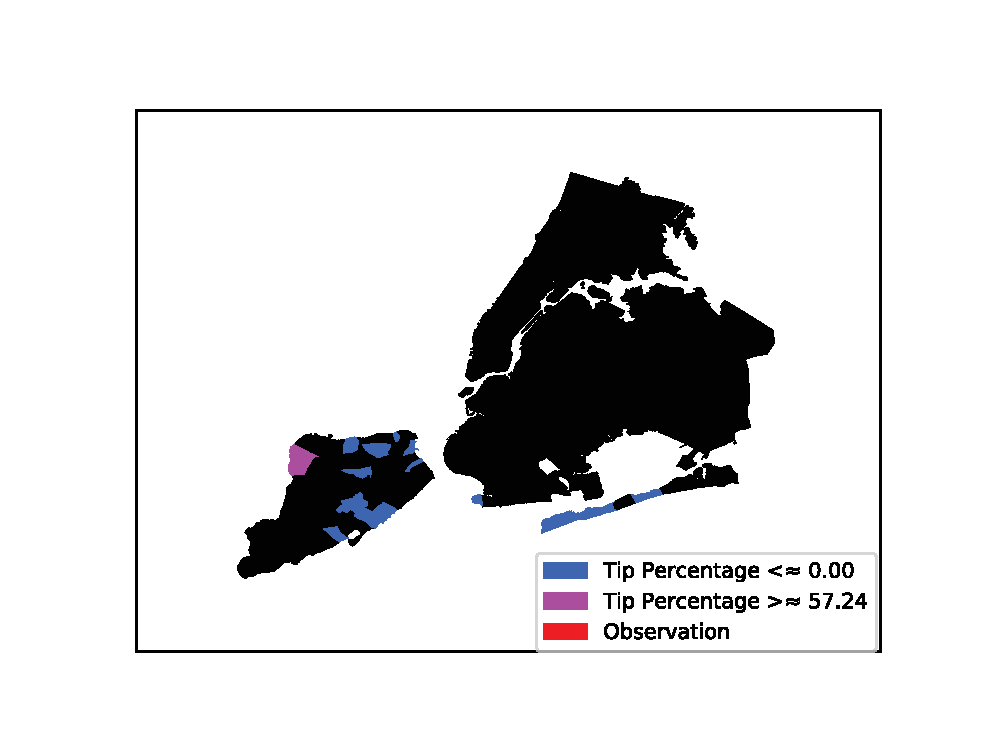
\includegraphics[width=\columnwidth]{images/spatial_explanation_example.eps}
%\caption{An example of spatial explanation}
%\label{fig:spatial_explanation_example}
%\end{figure}

\begin{figure}[t]
	\centering
	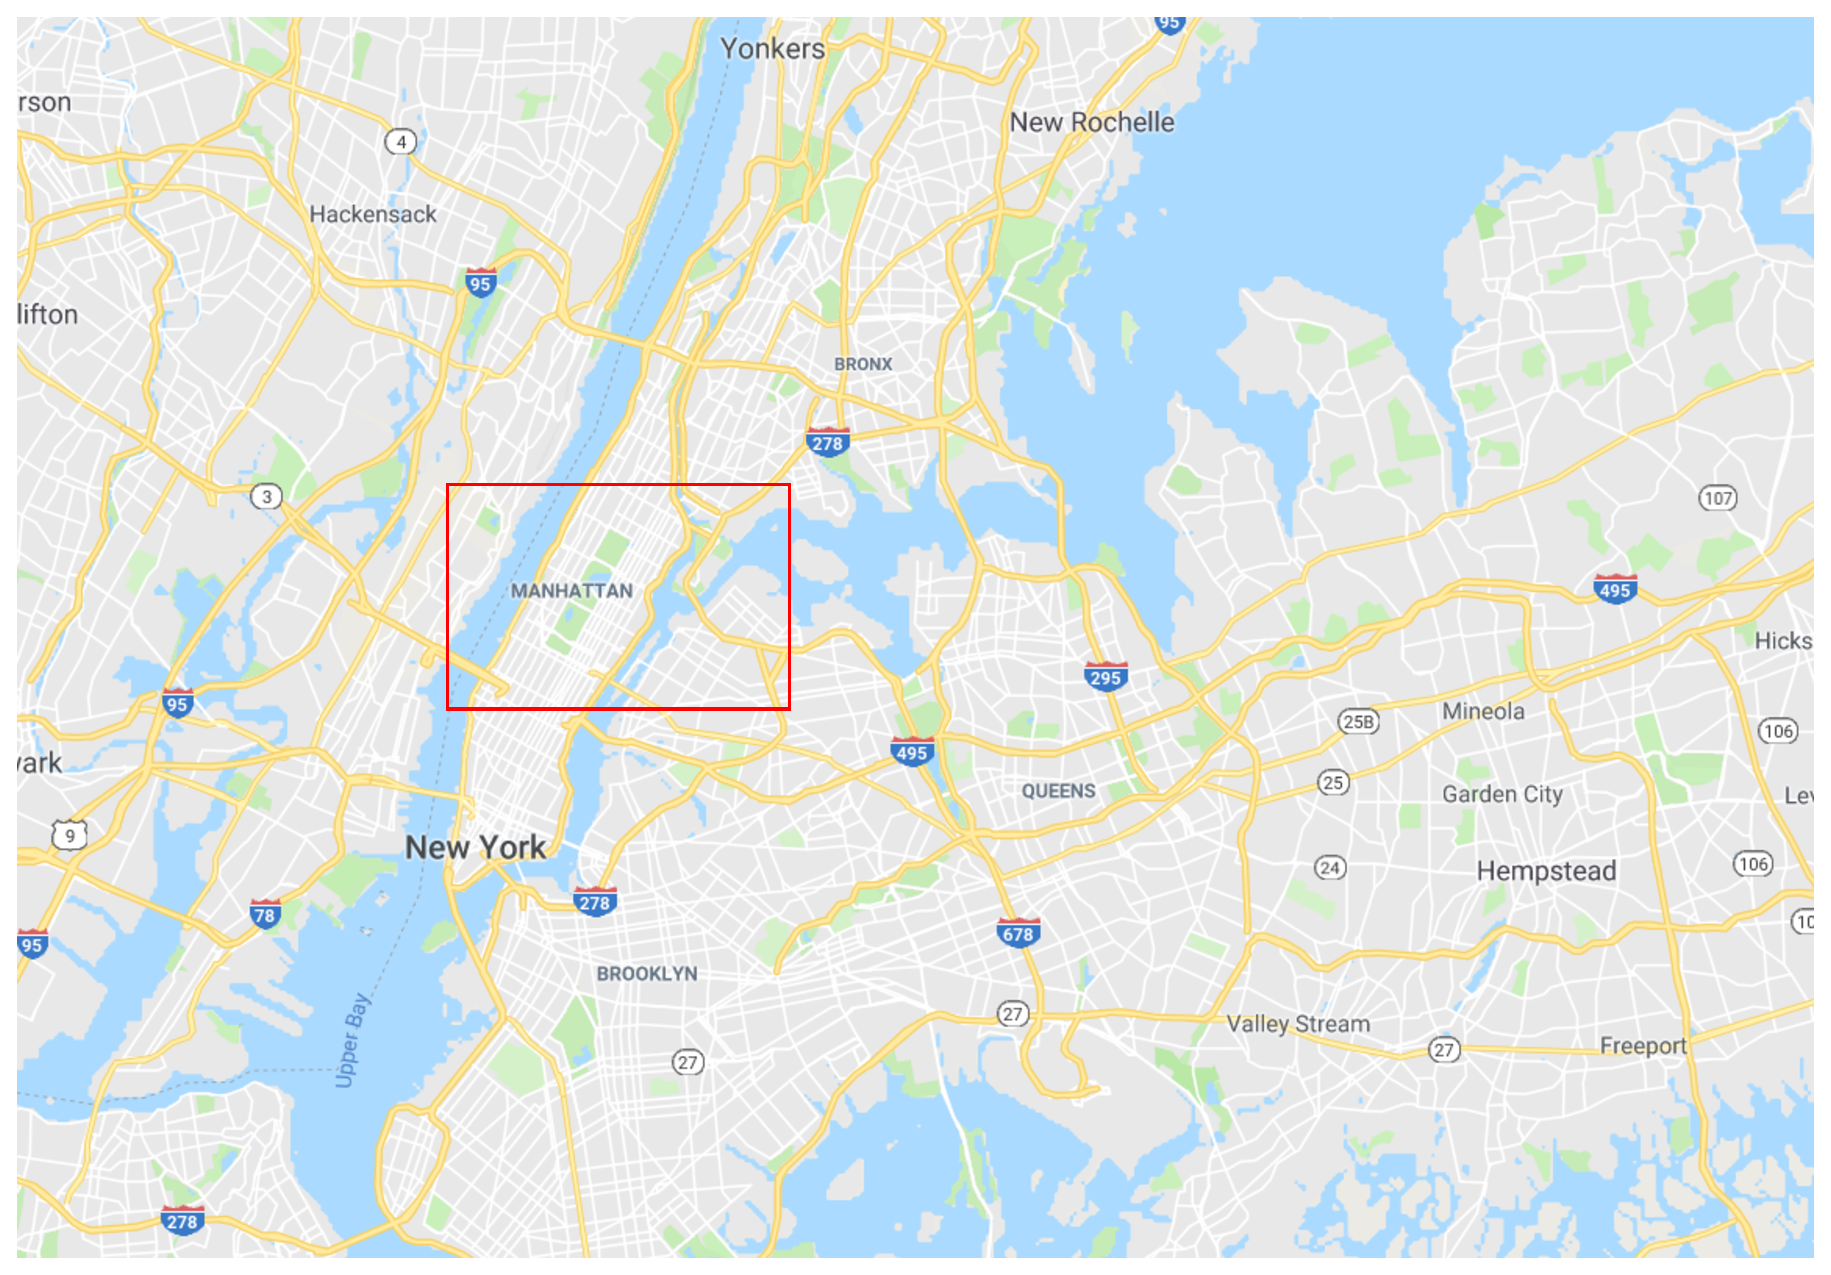
\includegraphics[width=0.46\textwidth]{images/spatial_explanation_map.eps}
	\caption{Spatial {\explanation} example}
	\label{fig:spatial_explanation_example}
\end{figure}

%{\bf Example.} 
Figure~\ref{fig:spatial_explanation_example} shows an example for a spatial {\explanation}. The red rectangle in the figure is a spatial {\explanation}. Such explanation consists of the data tuples whose drop-off locations are within the rectangle. The number of trips for this {\explanation} on 22nd and 23rd, Jan and the intensity, influence values are listed in Table \ref{table:intensity_influence_example}. We can notice that such {\explanation} has much higher intensity and influence than all the other {\explanation}s. It shows that considering spatial location can give us better {\explanation} for such {\fact}. 

%the heatmap for the value of $Q = q_1 / q_2$. It shows that the high values are located closely which means the {\fact} that the decreasing of the number of trips are caused by the trips that happen in some specific regions. Spatial aspect plays an important role in the {\fact} {\explanation} question. So the problem comes to how to detect these regions in a convenient and efficient way. In the following section, we will discuss our solution.

%The polygons painted purple show polygons in the candidate {\explanation} where the tip percentage is high, while polygons painted blue show candidate explanations where the tip percentage is low. It should be noted that $P$ has a high number of permutations. It is up to the approach to decide which polygons to include in the candidate explanation. For instance, hierarchical intervention may choose polygons in spatial proximity while aggravation may choose otherwise.
%\begin{figure}[t]
%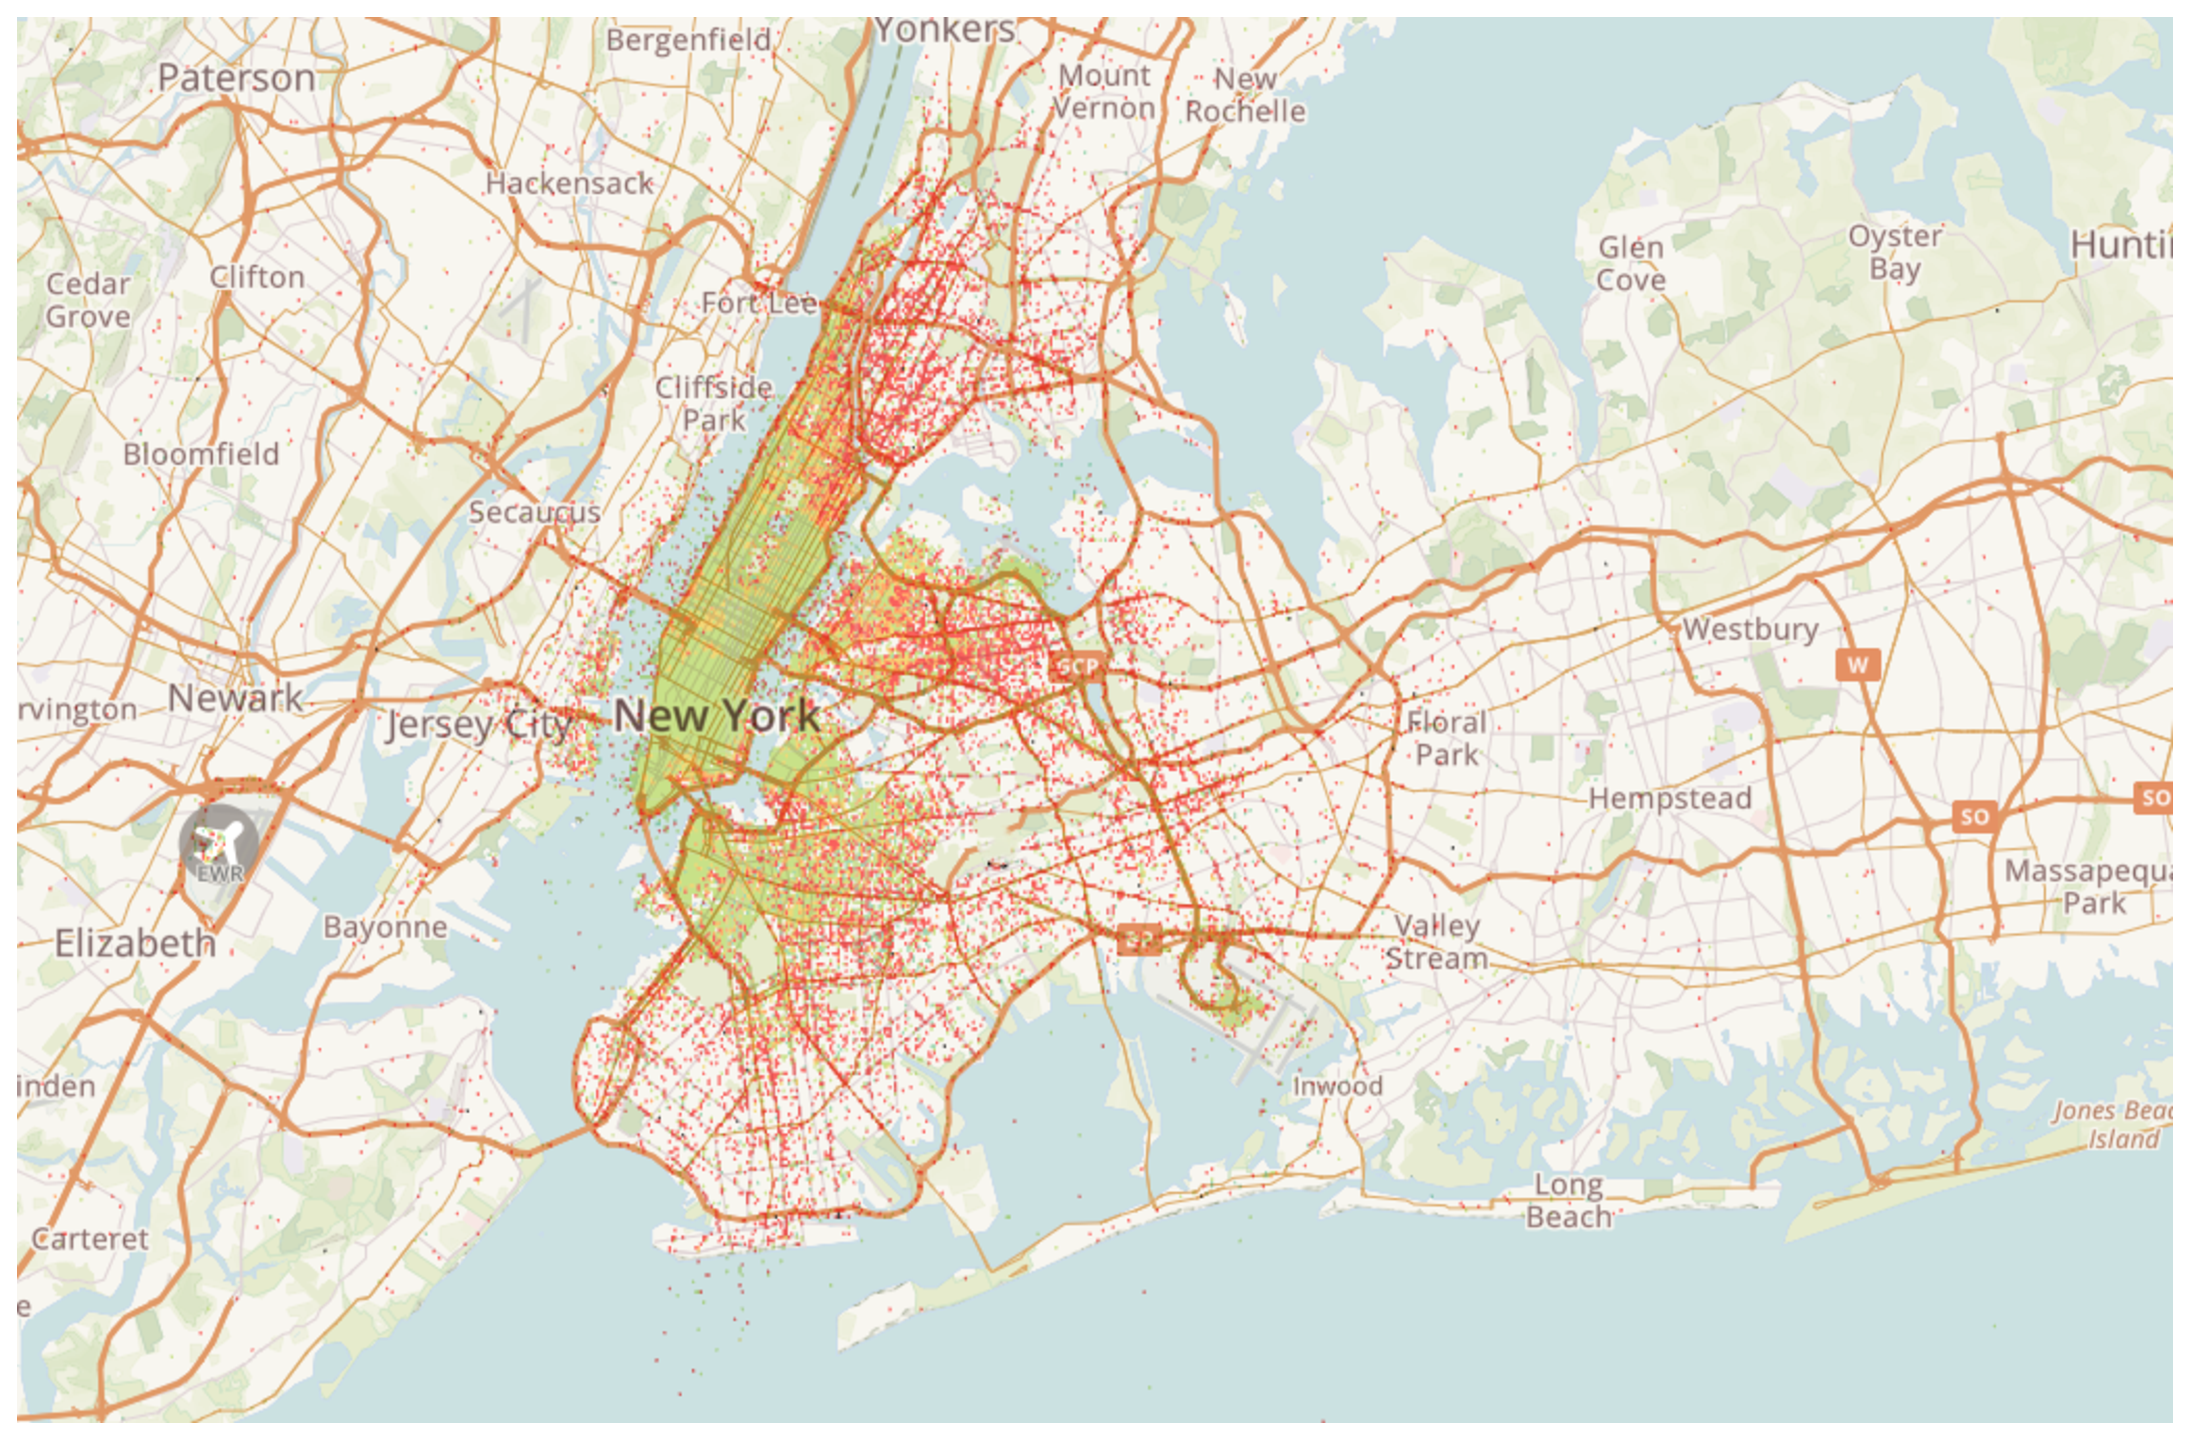
\includegraphics[width=\columnwidth]{images/scatter}
%\caption{Heatmap for NYC trips for January 2016}
%\label{fig:square_unit_grid}
%\end{figure}

%\my{Another interesting consideration when we are talking about spatial explanations is the density of the data. Fig.~\ref{fig:square_unit_grid} shows the heatmap for tip percentage with respect to pickup coordinates. It is interesting to observe that the explanations provided in Fig.~\ref{fig:spatial_explanation_example} are all areas with a low density of data. One of the reasons for this is because each approach takes some liberty with our definition of the taxonomy. Even though we defined $P$ to contain all permutations of polygons, an approach may use limited polygons, such as neighborhoods or zones. The way the explanation is ranked also plays a large role.}




% \section{Front End Visualization Tools}
% React\cite{reactjs} is a front end framework which originated in Facebook. The React framework allows interfaces to be designed using components. Each component has properties and a state. A component can have subcomponents. This makes it simpler to design interfaces which show consistent data across components. Some of the charts included in the interface make use of the eCharts library\cite{echarts}.

% MapBox\cite{mapbox} is a library for displaying maps. The maps provided by mapbox consists of tiles and vectors. Each tile represents a cube of the map while vectors are shapes which represent roads, buildings, etc. Deck.gl\cite{deckgl} is a library for creating an overlay on top of the map. Examples of overlays include scatterplots, cartograms etc. Matplotlib was also used for static plots for evaluation\cite{hunter2007matplotlib}.

% We have used all of these tools in a GUI for our framework. The details of the implementation can be found in Section~\ref{sec:implementation}






\section{Hierarchical intervention}
\label{sec:hei_intervention}
%\section{System Overview}
%\section{Star Schema}
%{\bf Star Schema.} 
%{\bf Star schema.} 

%\section{Hierarchical intervention}
%\label{sec:hei_intervention}
The first task is to find candidate spatial {\explanation}s, but
it is not trivial to generate candidate spatial {\explanation}s. 
Spatial data is continuous in the space, which makes it impossible to naturally divide data into buckets like what we have done for the attribute \emph{PayType}. 
For such type of attribute, one common solution is to partition based on value range. 
This solution makes sense for one-dimensional attributes. 
However, spatial data is continuous in 2-Dimensional space. 
A straight solution to partition data is to use grid cell, which is directly extended from the 1-dimensional's partition based on value range. 
This method suffers from the data skewness, which means that some grid cells are empty while some grid cells are super crowded. 
Another problem is to determine the number of partitions. 
In order to cope with these problems, we propose a solution called {\solution}. 

%\section{Introduction}
%This section details our approach called Hierarchical Intervention which is an extension of the intervention approach. 
%The idea behind hierarchical intervention is to improve the generated explanations by grouping spatially co-located polygons in the candidate set of explanations. The whole space is divided into a different number of partitions in several levels in pyramid manner. The highest level contains the entire space as one predicate, while each predicate in the lowest level contains one zone or a point.



%\subsection{Intervention approach with spatial support}
%
%Intervention is an approach inspired by the concept of influence. It builds on the aggravation approach(Section~\ref{sec:aggravation}). Intervention tries to measure how much our observations would change had our explanation not been present. Let $D$ be the dataset we are interested in. Let $Q$ be a function which returns the value of our observation given a dataset. Keeping our taxonomy in context, this means $Q$ returns the value of our aggregate observation query. Let $\phi$ be our candidate explanation. Let $\Delta_\phi \leftarrow \sigma_\phi(D)$. Let $D_\phi = D - \Delta_\phi$. The direction of our observation can either be \textit{high} or \textit{low} depending on whether we are interested in the greatest or least values of observation respectively. Our degree of candidate explanation by intervention, $\delta_{int}$, can then be expressed as,
%\begin{equation}
%\delta_{int}:=
%\begin{cases}
%-Q(D_\phi), & \text{if}\ direction=high \\
%Q(D_\phi), & \text{otherwise}
%\end{cases}
%\end{equation}
%
%We want the degree of candidate explanation by intervention to be higher the closer we are to the direction of the observation, therefore, we use the negative value when the direction is high. If the influence of the candidate explanation is high, it will result in a low observation value once the candidate explanation is removed from the dataset.
%
%Since intervention extends the idea presented by aggravation, it has similar issues when it comes to the number of permutations for candidate explanations. Similar to our approach in aggravation(Section~\ref{sec:aggravation}), we can reduce the number of permutations by bucketing the attributes. We can extend intervention for spatial observations and explanations the same way we did for aggravation. The set $P$ consists of distinct non-overlapping polygons in our dataset $D$. Let $s$,$t$ be the spatial attributes in $D$. Each tuple in $P$ has two attributes: $polygon\_id$, and $polygon$.

%\subsection{Hierarchical intervention overview}
%{\bf Main idea.} The proposed approach partitions the data spatially into a hierarchy. 
%The top level of the hierarchy consists of all the tuples in the data. 
%The lowest level of the hierarchy consists of each individual tuple. 
%Each cluster in the hierarchy forms a spatial predicate. 
%We harness this hierarchy to perform the {\aggravation} and {\intervention} approaches for a given fact. 
%Finally, we compare all the clusters in every level of the hierarchy to rank explanations.

%In order to get a better understanding of the spatial explanation approach, we will highlight our algorithm. 
We have designed our approach in the context of the programming paradigms provided by Apache Spark. 
The algorithm uses DataFrames to store each level in the spatial hierarchy. 
The leaf nodes are populated using {\aggravation}/{\intervention} operations. 
The {\aggravation}/{\intervention} values of the non-leaf nodes are populated using the data from children nodes. 
Since our technique uses memorization in a directed acyclic graph, it can be categorized as a dynamic programming approach.

%Figure~\ref{fig:steps} shows the hierarchical tree structure of the data. 
%Nodes with overlapping children are marked using a red dashed line. 
%The children of these nodes represent clusters of tuples which have some common points of intersection. 
%Since we want to build our graph bottom up, such overlaps present a concern. 
%We do not want to use tuples multiple times in our calculations.

% We represent each node in our hierarchy in a dataframe(Fig.~\ref{fig:steps}). The dataframe contains the id of the node($tid$), the id of the parent node($parent$), intervention, aggravation, aggregates of each attribute, and a column for intervention and aggravation for each aggregate query in our input. While dataframes look like traditional RDBMS tables, they have a few differences. Our solution exploits these differences to get more out of the system. In this case, we use the arbitrary number of columns in the dataframe to our advantage by representing the aggravation/intervention for each query in a separate column.

% In order to build the DAG bottom up, we want to use the values of aggravation and intervention in the children nodes to build up. At the beginning of the algorithm, we keep a record of the aggregates for the entire dataset. As mentioned before, we also have aggregates for each node in our dataframe. We can use these two values to calculate aggravation or intervention. For example, if our aggregate query was $SUM$ of an attribute and the node we are looking at consists of two child nodes, then the aggravation value would just be the sum of both the children. The intervention value would be the difference between the sum of the child nodes and the sum of the entire data. Using this approach we can build the explanations up using a left join on the parent and children dataframes.

Once we have built up our DAG one level, we still have tuples which contain incorrect data. These are the tuples with duplicates. Fig.~\ref{fig:steps} shows a representation of this scenario. In order to handle this case, we split our dataframe into two parts: one containing nodes with overlap bit, and one containing tuples without the overlap bit. The Dataframe with the tuples containing the overlap bit has the intervention and aggravation values recalculated. Finally, the split dataframes are merged together to give a final dataframe for the level in the hierarchy without and recounted values. This dataframe can be used for constructing the DAG up further iteratively till we reach the root node.

\begin{algorithm}
	\caption{Algorithm for Hierarchical Intervention}\label{alg:hieint}
	\begin{algorithmic}[1]
		\Procedure{Explain}{$tuples$}
		\State $input: \textnormal{tuples with spatial attribute}$
		\State $output: \textnormal{ranked spatial explanations}$
		\State $hierarchy \gets Cluster(tuples)$
		\Comment{Step 1}
		\State $dag \gets \textit{Create Dataframes from hierarchical levels}$
		\Comment{Step 2}
		\State $current\_level \gets \textit{Get last level from }dag$
		\State $AggravationIntervention(current\_level)$
		\State $current\_level \gets current\_level - 1$
		\While{$current\_level > 0$}
		\State $AggravationIntervention(current\_level)$
		\Comment{Step 3}
		\State $ResolveOverlaps(current\_level)$
		\Comment{Step 4}
		\EndWhile
		\State $explanations \gets Rank(dag)$
		\Comment{Step 5}
		\State \textbf{return} $explantions$
		\EndProcedure
	\end{algorithmic}
\end{algorithm}




\begin{figure*}[t]
	\centerline{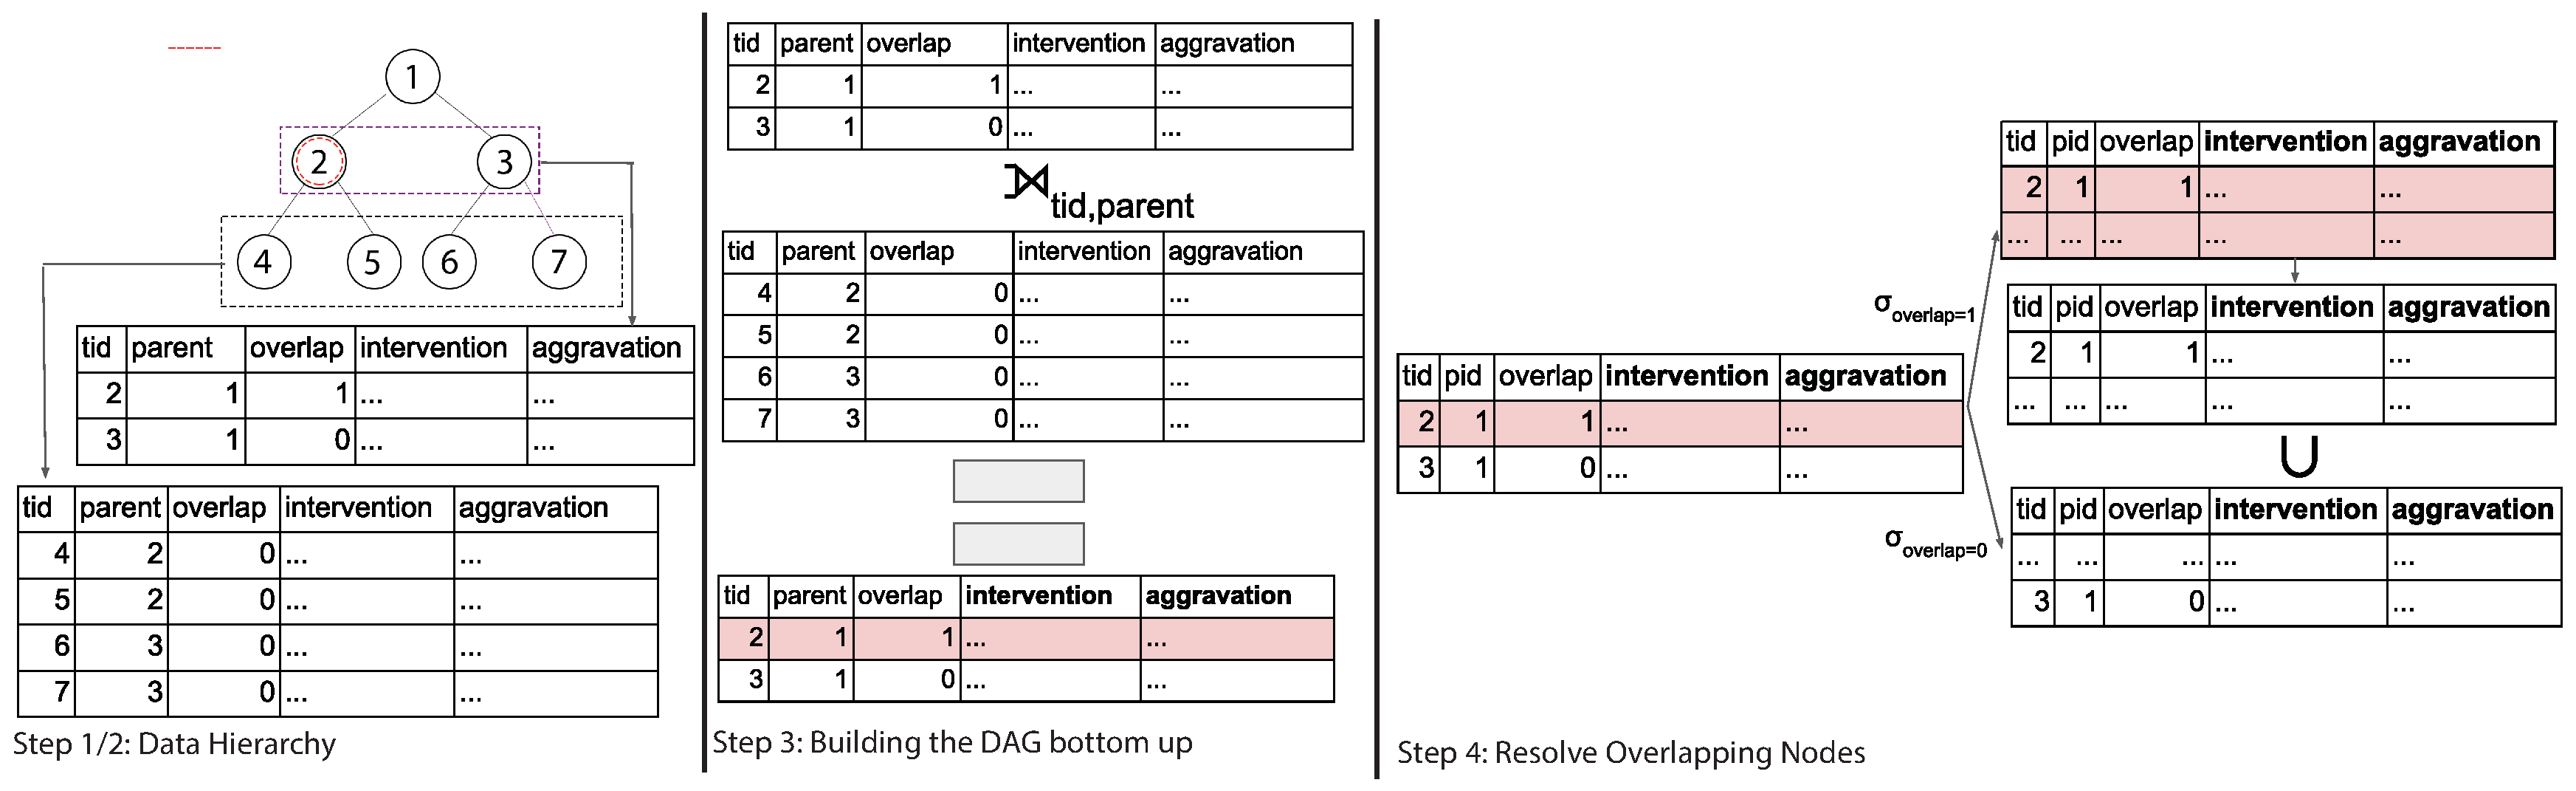
\includegraphics[width=0.95\textwidth]{images/steps}}
	\caption{Finding Spatial Explanation. The red dotted lines represent nodes which have children with overlapping tuples.}
	\label{fig:steps}
\end{figure*}


\subsubsection{Step1: Spatial Partitioning/Clustering}
Since it is hard to decide the granularity of the {\explanation}, our approach partitions the data spatially into a hierarchy. 
Figure~\ref{fig:steps} shows the hierarchical tree structure of the data. 
The top level of the hierarchy consists of all the tuples in the data. 
The lowest level of the hierarchy consists of each individual tuple. 
Each cluster in the hierarchy can be used as a predicate to form a spatial {\explanation}. 
In this way, {\explanation}s on different levels have different granularities. 
Several approaches can be used to cluster spatial data. The clustering method has a large impact on the resulting explanations. The impact of the clustering method will be studied in Section~\ref{sec:evaluation}.

%{\bf R-Tree} An R-Tree is a data structure which is commonly used for spatial data indexing. The idea behind the R-Tree is similar to the idea behind a binary tree i.e. It is faster to query data if it is stored in the form of a hierarchy\cite{guttman1984r}. In an R Tree, this hierarchy exists in the form of Minimum Bounding Rectangles(MBR). The top level of an R Tree consists of a set of MBRs which cover a large spatial area. Each MBR can now be subdivided into further MBRs which makes up the second level of the tree and so forth. At the leaf nodes of the tree, each node consists of a single object in our underlying data.


%{\bf R*-Tree} R* Tree is a variation of R-Tree\cite{beckmann1990r}. The objective of an R*-Tree is to minimize overlaps and coverage in an R-Tree. It also optimizes for margin and area. The idea behind R*-Tree which helps in achieving its objective is to use the perimeter of the MBR as a heuristic when splitting and creating R-Trees.

%{\bf K means} K means clustering is an algorithm designed to cluster a group of points \cite{macqueen1967some}. As the name suggests, the user decides the number of clusters that he/she wants. $K$ represents the number of clusters. The algorithm randomly selects $k$ seed points. The seed points can also be selected using a heuristic to improve the clustering. The points closest to each of the seed points form clusters. The k means algorithm is iterative. Which means it does not end there. The centroids of the clusters are used as new seed points and the process is repeated until the centroids are constant.


% TODO Add reference to greedy hierarchical clustering
% Let $D$ be our spatial dataset. Let $P$ be a set of distinct polygons over our dataset $D$. We define a set of distinct clusters of polygons $P_h$. The polygons can be clustered in many different ways but we used greedy hierarchical clustering because of its speed and relevance to the problem. Let $C$ be the set of centroids in $P$ i.e. $\forall p_i \in P$, $c_i$ is the centroid for $p_i$, where $c_i \in C$. We define a set of $n$ levels, $L = \{l_1, l_2,...,l_n\}$. We represent each centroid in $C$ on a cartesian plane where $x_i$ is the first dimension of the centroid $c_i$ and $y_i$ is the second dimension of the centroid $c_i$. Let $x_{min}$, $x_{max}$ be the minimum and maximum value for $x_i$ respectively. Let $y_{min}$, $y_{max}$ be the minimum and maximum values of $y_i$ respectively. There is a radius associated with each level in $L$. Let $r_i$ be the radius for level $l_i$ in $L$, We can define $r_i$ in general as,
% $$r_i = \frac{\sqrt{(y_{max}-y_{min})^2+(x_{max}-x_{min})^2}}{2^{i-1}}$$

% The set of clusters,$G_i$, for level $l_i$ can be defined as $G_i=\{p_k|(x_k^2 + y_k^2 < r_i^2)\}\forall p_k \in P$. Any possible set cover of $P$ in $G_i$ can now be considered for inclusion in $P_h$. One implementation of this approach is covered in Section~\ref{sec:hie_impl}


% \subsection{Hierarchical Greedy Clustering}
% Hierarchical Greedy Clustering is a popular algorithm in data visualizations because of its speed \cite{hgclustering}. The idea behind this algorithm is to randomly select points and create clusters around them.

% Let $D$ be our spatial dataset. Let $P$ be a set of distinct polygons over our dataset $D$. We define a set of distinct clusters of polygons $P_h$. Let $C$ be the set of centroids in $P$ i.e. $\forall p_i \in P$, $c_i$ is the centroid for $p_i$, where $c_i \in C$. We define a set of $n$ levels, $L = \{l_1, l_2,...,l_n\}$. We represent each centroid in $C$ on a Cartesian plane where $x_i$ is the first dimension of the centroid $c_i$ and $y_i$ is the second dimension of the centroid $c_i$. Let $x_{min}$, $x_{max}$ be the minimum and maximum value for $x_i$ respectively. Let $y_{min}$, $y_{max}$ be the minimum and maximum values of $y_i$ respectively. There is a radius associated with each level in $L$. Let $r_i$ be the radius for level $l_i$ in $L$, We can define $r_i$ in general as,
% $$r_i = \frac{\sqrt{(y_{max}-y_{min})^2+(x_{max}-x_{min})^2}}{2^{i-1}}$$

% The set of clusters,$G_i$, for level $l_i$ can be defined as $G_i=\{p_k|(x_k^2 + y_k^2 < r_i^2)\}\forall p_k \in P$. The algorithm for the implementation of this approach is covered in Section~\ref{sec:hie_impl}.

% Greedy Hierarchical Clustering turned out to have a drawback when we use it for explanations. It selects seed points randomly. This means that in each level, the clusters can be highly imbalanced. We compared this approach to K means(Voronoi partitioning)\cite{hartigan1979algorithm,aurenhammer2000voronoi}, R Tree\cite{guttman1984r} and R* Tree\cite{beckmann1990r}.

%The main idea behind the {\solution} approach is to help us in increasing the domain for our degree of explanation. 
%Since intervention is a subset of this approach, the domain is at least as large as that for intervention. After we have partitioned our data, each partition can be used as a predicate for aggravation and/or intervention.

\subsubsection{Step2: Hierarchical DataFrames Construction}
In our implementation of the system, we utilize the programming paradigm provided by Apache Spark. This involves using DataFrames for processing. Dataframes resemble tables in a traditional RDBMS. Each spatial {\explanation}in our spatial hierarchy is represented as a node in a tree. Each level of the tree is encapsulated as a DataFrame. Each node has an ID associated with it. Each tuple in our DataFrame is stored with the ID of the node that contains it, the ID of the parent node, a column representing the overlap bit, columns representing the aggregates of the attributes, columns representing the aggravation/intervention for each query in our observation, and a column for the final values of aggravation/intervention after evaluating the arithmetic operation that represents our observation. 

%The spatial hierarchy that we construct in step 1 of our algorithm is already a DAG since it takes the form of a tree. But for the next few steps, the DAG that we use is based on the DataFrames. Instead of calculating {\aggravation} and {\intervention} for each node DataFrames, we can reuse the values calculated in the leaf DataFrame for higher level DataFrames.

\subsubsection{Step3: Building up the DAG}
{\aggravation} and {\intervention} are very expensive operations. 
%In order to create a system for explanations which performs well, we need to reuse calculations. That's the main reason we constructed our DAG in the first place. 
In order to improve the performance of the system, we reuse the values calculated in the leaf DataFrame to compute the values for higher level DataFrames. 
%The intervention/aggravation values stored in one level of our DAG can be used one level above. 
We use the associative property of aggregate functions like sum and count to build our DAG bottom up. 
The bottom-up procedure can be implemented by using group and join operations in DataFrames. 
%The tuples at one level are grouped based on the parent id and left joined with the tuples at the parent level based on the node id and parent id of the child and parent dataframes respectively. 
The tuples at one level are grouped based on the parent id.  
Then the lower level DataFrame is left joined with the parent level DataFrame based on parent id of the child DataFrame and tuple id of the higher level DataFrame. 

\subsubsection{Step4: Overlap Resolution}
Our system is designed to work with arbitrary clustering algorithms. 
Some of the clustering algorithms like K-Means have no overlapping tuples in the clusters while others like R-Tree have partitions with overlaps. 
In this case, a node in the hierarchy can have children that share common data tuples. 
Then the computation of the value on the current node cannot be implemented by directly merging the results from its children. 
The way to handle the overlap cases is to store a bit value.
If a node has overlapped children, the overlap bit for this node is set to \emph{true}. 
%In our spatial hierarchy if a node has child nodes with overlapping points, the overlap bit for that node is set to $true$. 
%Using our build-up approach so far, these nodes contain inaccurate values of intervention and aggravation. Before building the DAG further up these values need to be fixed.
Due to the immutability of DataFrames, we create one more DataFrame for the nodes whose overlap bit is \emph{true}. 
In each level, nodes whose overlap bit is \emph{false} can reuse values from their children. Nodes in the DataFrame with \emph{true} overlap bit will be recomputed to get the correct values. 
Then the built-up procedure is resumed. 

%Depending on the type of spatial partitioning, some nodes in our DAG have incorrect values of aggravation/intervention stored in the dataframe. These are nodes where the overlap bit is $true$. 
%Since we are using dataframes, we cannot update individual tuples. Instead, we create two dataframes out of the original. One containing tuples where the overlap bit is true and one containing the rest of the tuples. 
%The aggravation/intervention and aggregates for the first dataframe are recalculated. Finally, both the dataframes are combined using union and the old dataframe is replaced with the new one in the DAG. Using this sequence of operations, we can reduce the number of calculations. Since our dataframe now contains accurate information, we can resume building the DAG further up.


\subsubsection{Step5: Ranking Explanations}
\label{sec:extending_hi}
In this step, the system accumulate the {\intensity} and {\influence} values for all the {\explanation}s on all levels. Their values of {\newvalue} will be computed and sorted. The top-K {\explanation} will be output as the final result. 

%In order to get the most out of Hierarchical Intervention, we introduce two new metrics: Intensity and Influence.
%
%\textbf{Intensity:}
%\label{sec:intensity}
%%What is relevance
%We define intensity as a metric which measures the standalone value of the explanation. The relevance metric borrows a lot from our definition of aggravation. It might be convenient to think of a web search engine when we are looking at the intensity metric. When we use a search engine, we provide a search term as a query. The search engine looks at all the pages in its database and returns the results in order of relevance. The top results in the search engine may not have a significant effect on the entire web if they were to be removed. However, the top result in the search engine has the highest relation to the data. For example, the top result for a search engine which uses tf-idf might be a page containing the highest frequency of the search term\cite{robertson2004understanding}.
%
%%Formal definition of relevance
%Let $D$ be our dataset. Let $\phi$ be our candidate explanation. Let $R$ be the function which maps our dataset to the value of our observation. Then we can define intensity as,
%$$intensity = |R(\sigma (D)) - R(\sigma_\phi (D))|$$
%
%\textbf{Influence:}
%\label{sec:influence}
%% What is influence
%We define influence as a metric which measures the value of the explanation compared to the entire dataset. The influence metric borrows from our definition of intervention. The influence metric measures how much the observation would be affected if we remove the data related to our explanation(the \textit{influence} of our explanation on the observation). We can use the analogy of the search engine again here. One of the earliest algorithms used by Google to rank web pages used links to other pages\cite{brin1998anatomy}. The page which was linked the most on a variety of websites was ranked higher. If you remove a highly relevant page, many other pages might not exist. Influence uses the same principle.
%
%%Formal definition of influence
%Let $D$ be our dataset. Let $\phi$ be our candidate explanation. Let $R$ be the function which maps our dataset to the value of our observation. Then we can define relevance as,
%$$influence = |R(\sigma(D)) - R(\sigma_{\neg \phi} (D)) |$$
%
%The greater the value of influence, the more its impact on the observation.
%
%Our evaluation metrics suggest that influence and intensity explain data in different ways. Explanations with higher influence tend to give predicates which cover a larger area while explanations with higher intensity tend to give predicates which cover a small area. We can balance out these two metrics according to the preferences of the observer. We define the \textit{explanation index}, $\epsilon$ as:
%$$\epsilon = \alpha \times influence + (1-\alpha) \times intensity$$
%$\alpha$ is the \textit{explanation coefficient}. It is a variable whose value is decided by the user.
%
%Explanations given by Hierarchical Intervention can be ranked on the basis of the explanation index.
